\chapter{Introdução}

O trabalho que está em desenvolvimento aborda a aplicação de arquiteturas de redes neurais em problemas de classificação e identificação de formas e objetos em imagens. Os integrantes do grupo utilizarão conceitos de redes neurais convolucionais (CNN) aplicados
a um conjunto de imagens da série \emph{Os Simpsons}, com o objetivo de identificar corretamente seus personagens principais. Além disso, serão utilizadas técnicas para interpretar e visualizar as características aprendidas pela da rede de forma a entender quais são as peculiaridades de cada personagem que a rede utiliza para sua classificação. Este texto apresenta as atividades desenvolvidas até o momento com base em uma breve discussão do uso de camadas convolucionais para aplicações em imagens, assim como técnicas para utilização de redes pré-treinadas (\textit{transfer learning}) e interpretação dos resultados da aplicação da rede.

\chapter{Redes Neurais Convolucionais Aplicadas ao Processamento de Imagens}

As redes neurais convolucionais foram desenvolvidas para trabalhar com dados multidimensionais, como imagens 2D coloridas ou textos escritos ao longo do tempo. Nesse contexto, as CNN apresentam excelente desempenho e acurácia na classificação de padrões, uma vez que
sua arquitetura explora a localidade espacial da relação entre elementos adjacentes nesses dados \cite{lecun2015deep}.

Algumas características arquiteturais são de grande importância para o bom funcionamento das CNN: 
\begin{itemize}
\item as camadas convolutivas não são totalmente conectadas (ao contrário das MLPs);
\item os pesos sinápticos são compartilhados entre os neurônios de uma mesma camada convolucional;
\item há a interpolação de múltiplas camadas convolucionais com camadas \emph{pooling} \cite{lecun2015deep}. 
\end{itemize}

Uma camada convolucional possui diversos hiperparâmetros, como o número de unidades (neurônios ou filtros), tamanho da janela de filtro (kernel), tamanho de passo de varredura (\textit{skipping} ou \textit{strides}) e tipo de funções de ativação \cite{cirecsan2011high}. Em termos matemáticos, a fórmula de aplicação do processo de convolução para as camadas convolutivas de uma CNN pode ser expressada como:

\begin{equation}
    M_{x}^{n} = \frac{M_{x}^{n-1} - K_{x}^{n}}{S_{x}^{n} + 1} + 1
\end{equation}

\begin{equation}
    M_{y}^{n} = \frac{M_{y}^{n-1} - K_{y}^{n}}{S_{y}^{n} + 1} + 1
\end{equation}

Onde M é o número de neurônios da camada; K o tamanho da janela e S o tamanho do passo de varredura ou \textit{stride}. As redes convolucionais simulam aplicação de um filtro dentro da imagem por meio de uma convolução 2D \cite{behnke2003hierarchical}. A figura \ref{fig:cnn-example} demonstra essa aplicação:

\begin{figure}[h!]
    \caption{Processamento de uma rede neural com convolução 2D}
    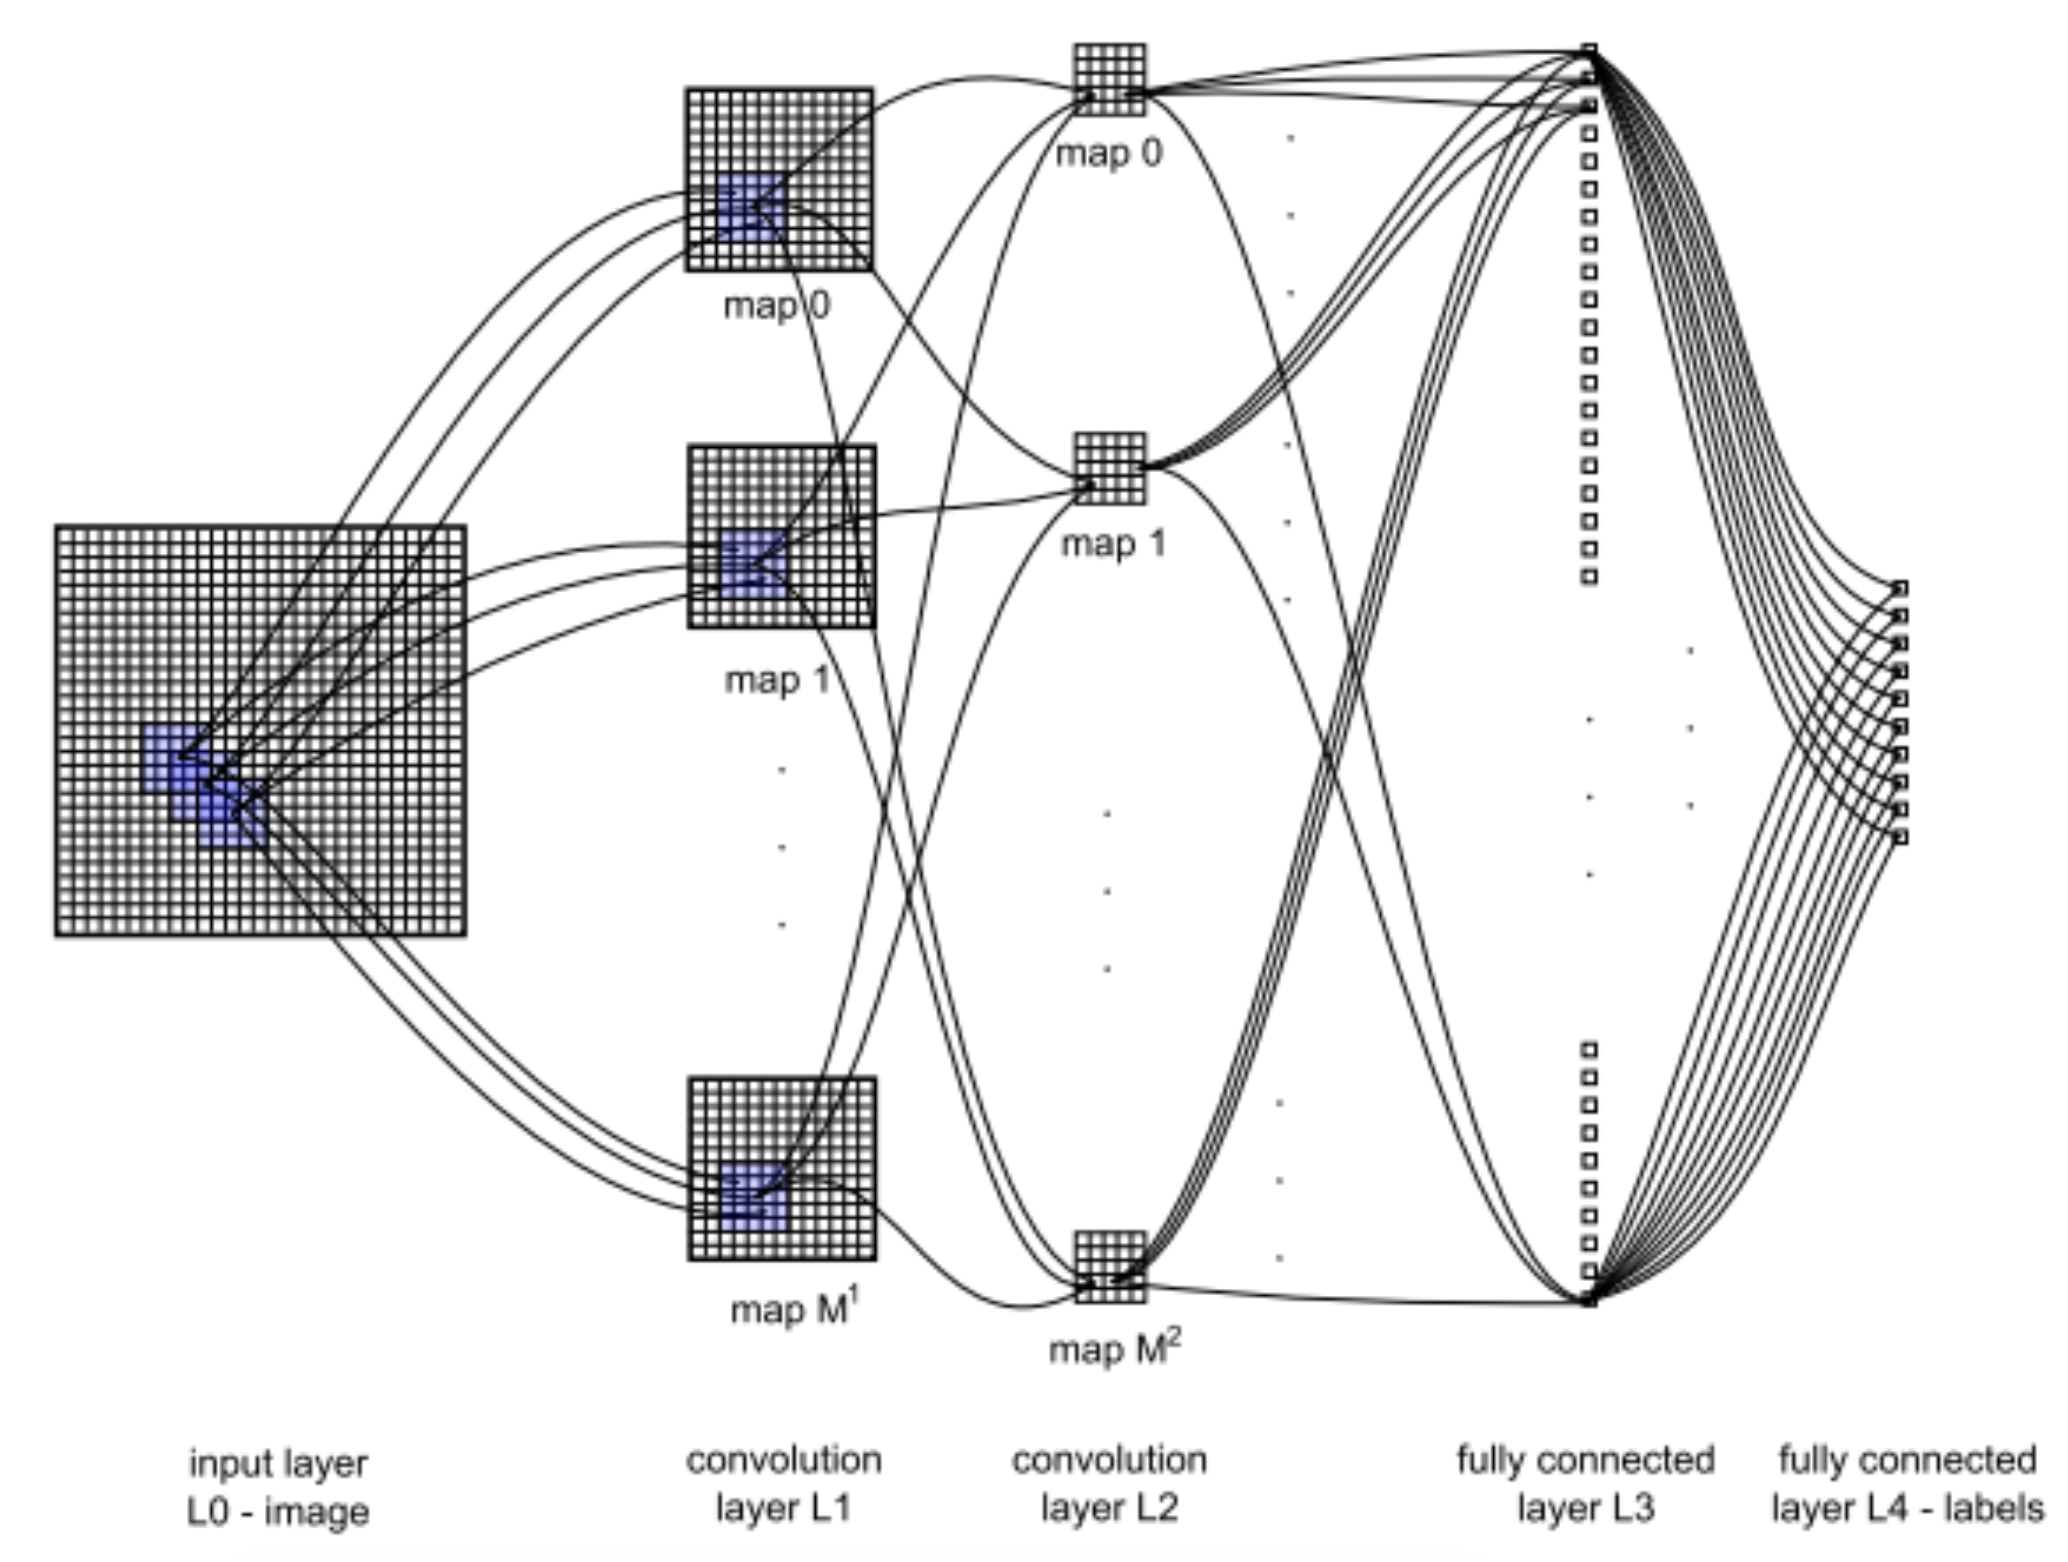
\includegraphics[width=0.8\textwidth]{cnn-example.png}
    \centering
    \label{fig:cnn-example}
\end{figure}

Vale destacar que, na figura \ref{fig:cnn-example}, as janelas azuis simulam a aplicação das camadas convolucionais. Por exemplo, na primeira camada são aplicadas janelas 5x5 na imagem original e sua saída são imagens também 2D mas de tamanho reduzido. É fácil observar que a saída de uma camada convolucional em uma imagem é um conjunto de imagens de medidas menores que a imagem original \cite{cirecsan2012multi}. Em seguida, é possível que sejam  utilizadas outras camadas convolucionais para identificação de outros padrões.

A vantagem de redes convolucionais sobre filtros convolucionais tradicionais (como os que identificam bordas) é que as redes convolucionais são capazes de mapear relações locais com não-linearidades dentro da imagem, devido a não-linearidade presente nas funções de ativação \cite{leen1995data}. Isso permite com que a rede identifique mais facilmente curvas e padrões os quais os filtros convolucionais tradicionais
apresentam dificuldades.

Existem diversas funções de ativação utilizadas em redes convolucionais, contudo a mais comum é a ReLU \cite{lecun2015deep}, a qual pode ser expressa como ReLU(x) = max(0,x). Essa função de ativação apresenta vantagens em relação a outras possíveis alternativas pois simplifica o cálculo da derivada (o caso x<=0 e 1 caso contrário) e o treinamento da rede por retropropagação \cite{leen1995data}.

O treinamento de camadas convolucionais é muito semelhante ao de camadas totalmente conectadas, ou seja, é por meio da retropropagação do erro da rede e consequente ajuste dos pesos de seus neurônios. Para isso, é necessário o cálculo das derivadas parciais da função de erro em relação aos pesos sinápticos.

Por fim, outra estrutura interessante de uma CNN são as camadas de \textit{pooling}. Essas camadas são utilizadas para a redução do tamanho das imagens 2D resultantes da aplicação das camadas convolucionais. Existem muitas possibilidades de \textit{pooling}, dentre as quais se destacam a média (\textit{average}), máximo (\textit{max-pooling})  e mínimo (\textit{min-pooling}). Essa redução de dimensionalidade é útil para síntese de informação \cite{cirecsan2011high} e identificação com maior facilidade de relações locais.

\chapter{Redes Pré-treinadas (\textit{Transfer Learning})}

\textit{Transfer Learning} (transferência de conhecimento) é uma técnica de aprendizado de máquina em que uma rede treinada sobre um dado
conjunto de dados específico para executar uma determinada tarefa é utilizada como ponto de início para o treinamento da execução de uma outra tarefa sobre um outro conjunto de dados. Para Redes Neurais Convolucionais, por exemplo, uma rede treinada para classificar determinadas imagens segundo algum critério de similaridade pode ser utilizada como ponto de partida para o treino de classificação de outras imagens.

As primeiras camadas de uma rede neural treinada para o reconhecimento de imagens coloridas sempre tem o comportamento de Filtros de \textit{Gabor} ou Cores (“\textit{Blobs}”) \cite{yosinski2014transferable}. Portanto podem ser facilmente reutilizadas para qualquer rede neural convolucional que lida com imagens coloridas como entrada. Já as últimas camadas têm características mais específicas.

Para essa e outras aplicações, o modo mais convencional de se inicializar uma rede neural utilizando transferência de conhecimento consiste em: 1) utilizar as primeiras camadas de uma rede neural já treinada; 2) destreinar as últimas camadas, iniciando-as com pesos aleatórios \cite{yosinski2014transferable}. Isso garante que os classificadores (últimas camadas) sejam reinicializados. 

A rede obtida será treinada com o novo conjunto de dados, e sua parametrização pode possibilitar o congelamento ou não de suas primeiras camadas. Se esse conjunto de dados for muito pequeno e o número de parâmetros for grande, não congelar as primeiras camadas pode causar sobreajuste. Caso contrário, a rede não terá uma porcentagem de acerto tão alta quanto se as camadas forem descongeladas.

%A transferência de conhecimento melhora não só o treino de i pequenos como de grandes também.

Outro ponto importante na transferência de conhecimento é a natureza das redes neurais. A eficácia dessa técnica diminui quanto maior a diferença entre as predições das duas redes. Mas com um conjunto de dados limitado, a transferência de conhecimento ainda é superior a reinicializar a rede com pesos aleatórios.

\chapter{Interpretando o Aprendizado de uma CNN}

Existem muitas técnicas para interpretar o aprendizado das redes convolucionais. Uma das mais comum é ilustrar o resultado da aplicação de camadas convolucionais nas imagens e tentar presumir o papel de cada camada no funcionamento da rede \cite{chollet2017deep}.

\begin{figure}[ht]
    \caption{Bloco básico para montagem de uma rede neural recorrente da categoria LSTM}
    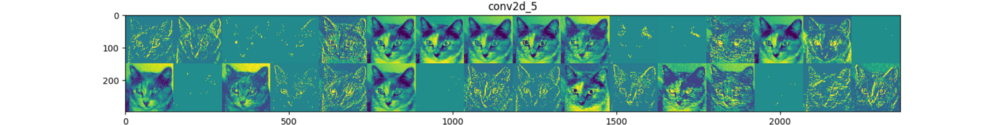
\includegraphics[width=\textwidth]{conv-cats}
    \centering
    \label{fig2}
\end{figure}

A imagem \ref{fig2} ilustra o resultado de uma primeira camada convolucional. Note que essa camada pode ser interpretada como uma camada para identificação de bordas na imagem original.

Outra técnica importante é o \textit{Deconvolutional Network} \cite{zeiler2014visualizing}, como o próprio nome já indica, redes deconvolucionais fazem exatamente o oposto das redes convolucionais tradicionais. Esse tipo de rede aplica uma convolução inversa nos resultados das camadas convolucionais. Além disso, também são utilizadas camadas de \textit{unpooling} que tentam aumentar a dimensionalidade das imagens, ainda que de modo aproximado \cite{zeiler2014visualizing}. Essa aproximação depende do \textit{pooling} usado na rede original dado que os \textit{max-pooling} não apresentam inversas. Logo, o que se faz é repetir o máximo de local para os \textit{pixels} da janela.

O resultado de uma \textit{DeconvNet} não é a imagem reconstituída totalmente, mas sim uma representação da imagem original, onde os \textit{pixels} mais relevantes ficam em maior destaque, como pode-se ver na figura \ref{fig:cnn-visualization}.

\begin{figure}[h]
    \caption{Visualização dos \textit{feature maps} de três imagens diferentes \cite{zeiler2014visualizing}}
    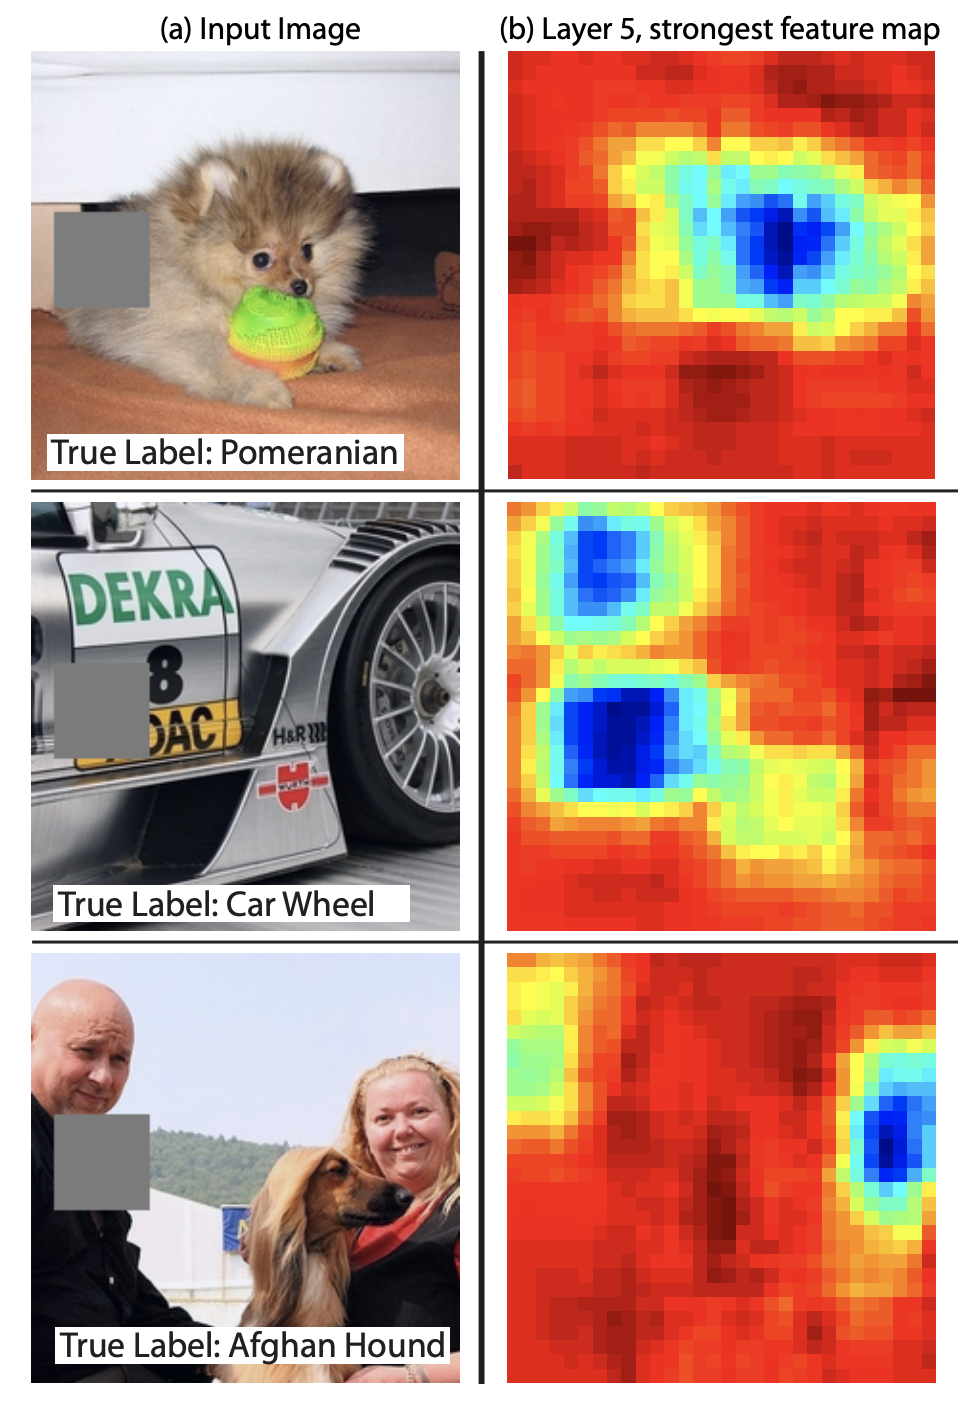
\includegraphics[width=0.6\textwidth]{cnn-visualization}
    \centering
    \label{fig:cnn-visualization}
\end{figure}

Por fim, uma das últimas técnicas mais importantes é o \textit{Layer Wise Relevance Propagation}, em que se utiliza os pesos sinápticos para calcular a importância dos \textit{pixels} da imagem original \cite{chollet2017deep}. O resultado da aplicação dessa técnica é uma imagem onde são mantidos apenas os \textit{pixels} relevantes para a classificação da imagem. Os demais \textit{pixels}, os quais não ativam a classificação, são “descartados” devidos a uma normalização empregada por essa técnica.

\chapter{Andamento dos ensaios}

Foram realizados diversos testes com a base dos \textit{Simpsons} para identificar os personagens principais. Inicialmente foi realizado um \textit{transfer learning} com a VGG16, onde foram retreinadas uma camada densa de 1024 neurônios e uma camada de saída com 18 neurônios (18 é o número de personagens na base de teste).

A acurácia dessa primeira rede foi de mais de 96\%, conseguindo identificar com êxito praticamente todos os personagens da animação.

O grupo agora planeja repetir os testes para as CNN \textit{InceptionV3} e \textit{ResNet50} e comparar os resultados. Além disso, também serão utilizadas técnicas de interpretabilidade de redes convolucionais na tentativa de entender quais aspectos dos personagens a rede identifica com maior facilidade. 

\chapter{Análise de temas}

Segue a tabela de análises que cada integrante irá fazer sobre tema dos demais grupos:

\begin{table}[h]
\begin{tabular}{|l|l|p{11cm}|}
\hline Aluno & Grupo & Tema \\
\hline Bruno & 9 & Análise de sentimento em avaliações de filmes no site imdb.com \\
\hline Gabriel & 1 & Classificação de placas de trânsito com redes neurais \\
\hline Lucas & 6 & Comparação entre o Gradiente Descendente e abordagens baseadas em enxame no treinamento de Redes Neurais em problemas de regressão. \\
\hline Vivian & 7 & Extração de características de imagens de Redes Neurais Convolucionais para inferir a posição espacial de objetos na imagem \\
\hline
\end{tabular}
\end{table}
